\documentclass[a4paper, 12pt]{article}

\usepackage[T2A]{fontenc}
\usepackage[english, russian]{babel}
\usepackage[top=2cm,bottom=3cm,left=1.5cm,right=1.5cm]{geometry}

% Пакет для расширения возможностей
% работы с формулами
\usepackage{amsmath}

% Расширение набора
% математических символов
\usepackage{amsfonts}
\usepackage{amssymb}

% Подключим пакет, отвечающий
% за изображения
\usepackage{graphicx}

\usepackage{indentfirst}

\graphicspath{ { ./images/ } }

% Попробуем подвигать текст вручную
% (тут мы будем двигать на титульном листе,
% но аналогичные операции будут работать
% везде в теле документа)
\begin{document}

\title{Отчёт о выполнении лабораторной работы 1.1.1 \\
Определение систематических и случайных погрешностей при измерении удельного сопротивления нихромовой проволоки}
\author{Новиков Александр, Б03-603}
\maketitle

\section{Аннотация}
В работе измеряется удельное сопротивление тонкой проволоки круглого сечения,
изготовленной из нихромового сплава.

Используется метод измерения сопротивления через
определение углового коэффициента наклона зависимости напряжения на проволоке от тока
через неё, измеряемых с помощью аналоговых и цифровых вольтметров и амперметров.

Геометрические размеры образца измеряются с помощью штангенциркуля и микрометра. 

\section{Теоретические сведения}
Удельное сопротивление материала проволоки круглого сечения, изготовленной из однородного материала и имеющей всюду одинаковую толщину, может быть определено по формуле:
\begin{equation}
    \rho = \frac{R_\text{пр}}{l} \frac{\pi d^2}{4}
    \label{mainformula}
\end{equation}
где $R_\text{пр}$ --- сопротивление измеряемого отрезка проволоки, $l$ --- его длина, $d$ --- диаметр проволоки.

Из закона Ома сопротивление можно найти, зная напряжение на проволоке и силу
тока, проходящего через неё, по следующей формуле:
$$R=\frac{U}{I}$$.

Из-за неидеальности вольтметра и амперметра возникает поправка, вызванная
параметрами приборов. Для измерения мы будем использовать схему, приведённую
на рис. \ref{fig:scheme}.

На схеме вольтметр правильно измеряет напряжение на проволоке, но
амперметр измеряет не только ток, прошедший через проволоку, но и ток, прошедший
через вольтметр.

Расчитаем поправку. Пусть $U$ и $I$ --- показания вольтметра
и амперметра соответственно. Тогда $R_1=U/I$.

Искомое сопротивление $R$:
\begin{equation}
\label{scheme1_bias}
R=R_1\frac{R_V}{R_V-R_1}=\frac{R_1}{1-(R_1/R_V)} 
\approx R_1\left(1+\frac{R_1}{R_V}\right)
\end{equation}

\begin{figure}
	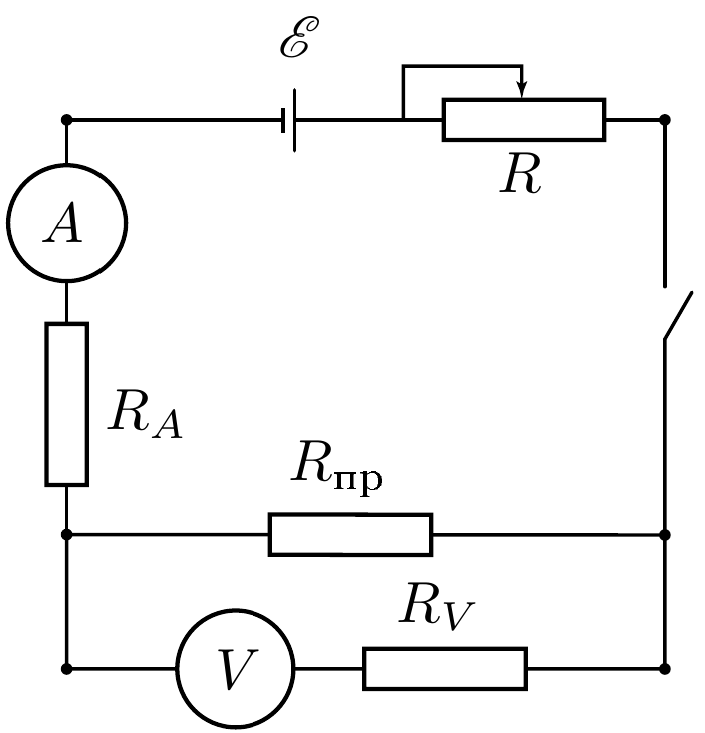
\includegraphics[width=0.4\textwidth]{images/scheme}
	\centering
	\caption{Схема для измерения сопротивления при помощи вольтметра и амперметра.}
	\label{fig:scheme}
\end{figure}

\section{Методика измерений}

\subsection{Приборы}
\begin{itemize}
\item Штангенциркуль: $\Delta {d_\text{шт}} = 0{,}05$ мм.
\item Микрометр: $\Delta {d_\text{мк}} = 0{,}01$ мм.
\item Вольтметр: стрелочный М2051, цена деления 5 мВ, предел 0{,}75 В, $R_V=5$ кОм, \\
$\Delta U_V = 5$ мВ.
\item Амперметр: цифровой GDM-8245, погрешность $\pm(0{,}03\% + 4 \text{ ед.})$, предел 2 А, $R_A=1{,}4$ Ом,
$\Delta I_A = 0{,}1$ мА.
\item Нихромовая проволока с контактами: $\Delta l = 2$ мм.
\end{itemize}

\subsection{Процедура измерений}
Диаметр проволоки измерялся на нескольких участках микрометром и
штангенциркулем. Показания штангенциркуля ($d_\text{шт}=0{,}29$ мм) существенно
отличались от показаний микрометра ($d_\text{мк}=0{,}37$ мм), что указывает на
систематическую погрешность штангенциркуля (возможно, сбитый нониус).
При измерении нулевой длины на штангенциркуле показание было равно $-0{,}1$~мм,
что подтверждает гипотезу о сбитом нониусе.
Для дальнейших расчётов использовались данные микрометра.

Для трёх длин проволоки ($l=20$, $30$, $50$ см) снималась вольт-амперная
характеристика. Для каждой длины получено по 9 точек в сторону увеличения напряжения
и по 6 точек в сторону уменьшения.

\begin{figure}
	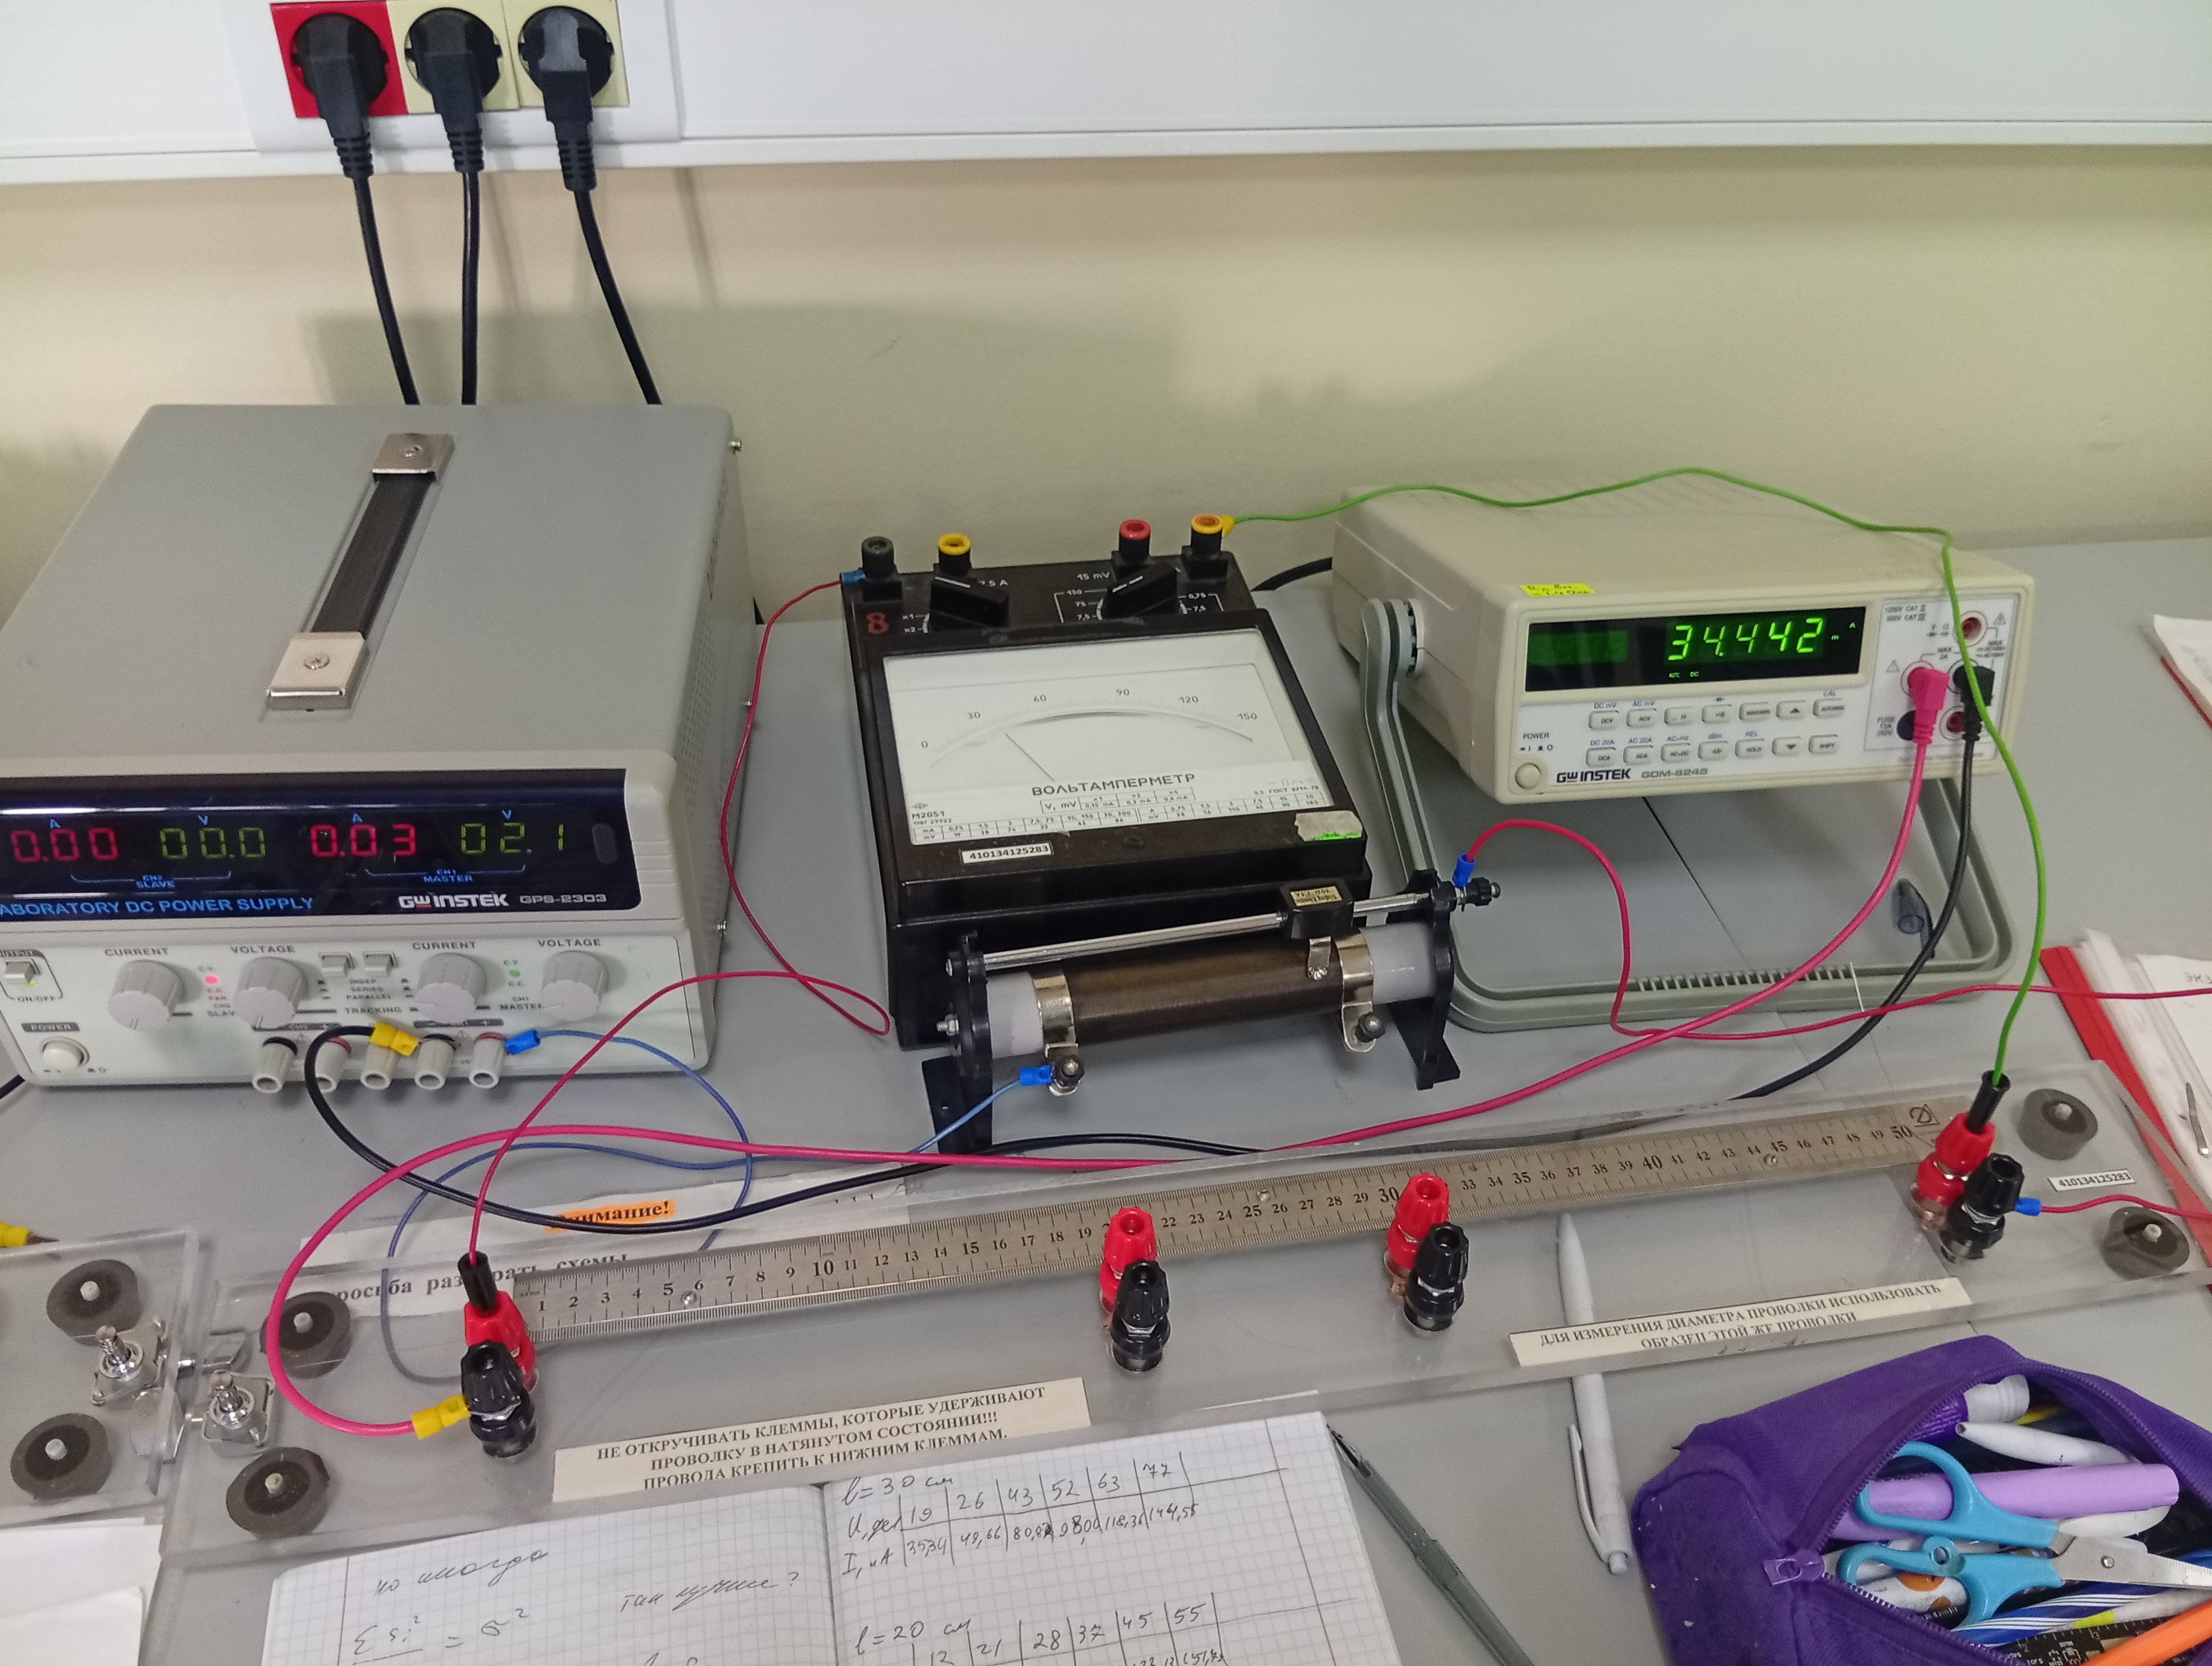
\includegraphics[width=0.8\textwidth]{images/installation}
	\centering
	\caption{Установка.}
	\label{fig:installation}
\end{figure}

\section{Результаты измерений}

\subsection{Диаметр проволоки}
Среднее значение диаметра по данным микрометра:
$\overline{d_\text{мк}} = 0{,}3678$ мм, стандартное отклонение
$\sigma_{d_\text{мк}} = 0{,}0044$ мм, случайная погрешность среднего
$\sigma_{\overline{d_\text{мк}}} = 0{,}0015$ мм. С учётом инструментальной
погрешности микрометра полная погрешность
$\sigma_{d_\text{мк}}^{\text{полн}} \approx 0{,}01$ мм. Окончательно:
\[
d = (0{,}37 \pm 0{,}01)\ \text{мм}, \qquad \varepsilon_d = 2{,}7\%.
\]

\begin{figure}
	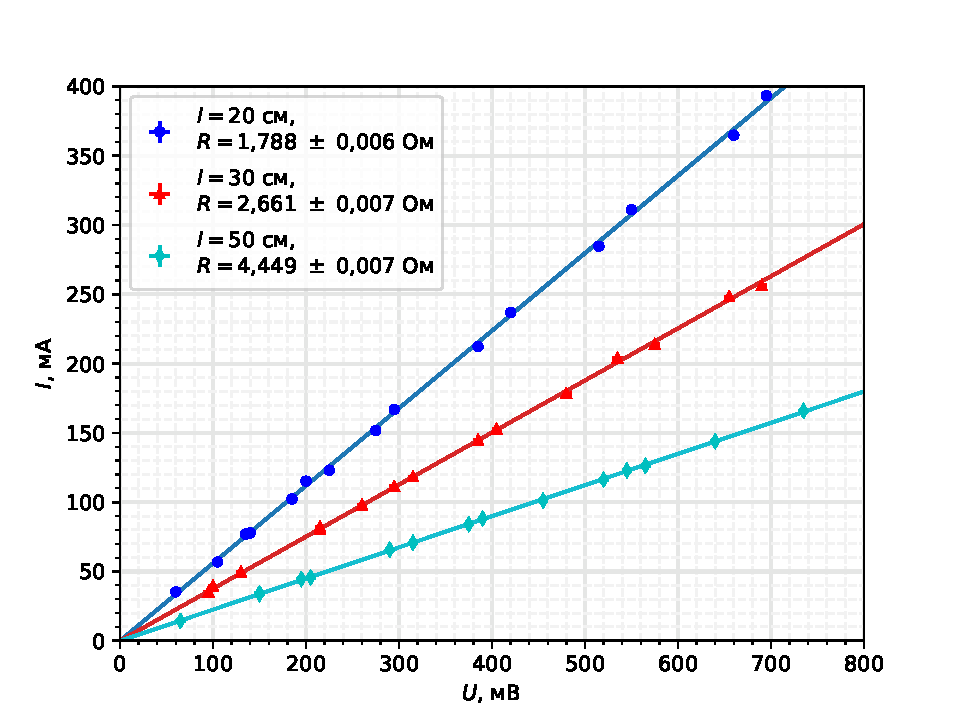
\includegraphics[width=\textwidth]{images/graph}
	\centering
	\caption{Вольт-амперные характеристики проволоки в зависимости от длины её отрезка.}
	\label{fig:graph}
\end{figure}

\subsection{Сопротивление проволоки}
Вольт-амперные характеристики и их линейная аппроксимация приведены
на рис. \ref{fig:graph}.
По графику видно, что экспериментальные данные с достаточно хорошей точностью
ложатся на теоретическую прямую $I = U/R_\text{изм}$.

Пользуясь методом наименьших квадратов, найдём сопротивление,
сопротивление проволоки с учетом поправки, случайную, систематическую и общую погрешности,
и занесём результаты в таблицу \ref{tab:resistance}.

Можно видеть, что основной вклад в результат вносят систематические погрешности.
Фактическая погрешность лежит в пределе двух-четырёх стандартных отклонений
и несёт систематический характер.
Также сопротивление проволоки с учетом отличается от измеренного в пределах погрешности.

\begin{table}[tbp]
    \caption{Результаты измерений сопротивления проволоки.}
    \begin{tabular}{|l|l|l|l|l|l|}
    \hline
    $l$, см & $R$, Ом  & $R_\text{изм}$, Ом & $\sigma_{R_\text{изм}}^{\text{случ}}$, Ом & $\sigma_{R_\text{изм}}^{\text{сист}}$, Ом & $\sigma_{R_\text{изм}}$, Ом \\ \hline
    20      & 1{,}7882 & 1{,}7875           & 0{,}0062                                  & 0{,}0129                                  & 0{,}0143                    \\ \hline
    30      & 2{,}6628 & 2{,}6614           & 0{,}0072                                  & 0{,}0193                                  & 0{,}0206                    \\ \hline
    50      & 4{,}4533 & 4{,}4493           & 0{,}0069                                  & 0{,}0304                                  & 0{,}0312                    \\ \hline
    \end{tabular}
    \centering
    \label{tab:resistance}
\end{table}

\subsection{Удельное сопротивление проволоки}
По формуле \ref{mainformula} находим удельное сопротивление материала проволоки
и его погрешность, используя найденные значения $R$.
Усредним результаты по трём длинам проволоки, получим:
$$\rho = (0{,}946 \pm 0{,}039) \times 10^{-6} \, \text{Ом} \cdot \text{м, } \epsilon_\rho = 4{,}12\%$$

\section{Заключение}

В работе удалось получить значение удельного сопротивления нихромовой проволоки
с точностью $\sim4{,}12\%$. Табличные значения удельного сопротивления лежат в диапазоне 
$\rho_{\text{табл}}=0{,}97...1{,}14 \cdot 10^{-6}\ \text{Ом} \cdot \text{м}$ в зависимости от
состава. Измеренные значения почти попадают в этот диапазон.

Существенно точность измерения снижается из-за высокой погрешности измерения
диаметра проволоки, для более точного измерения требуется или более точные
измерительные приборы, чем микрометр или штангенциркуль, или более толстая
проволока.

\end{document}